% !TEX root = ../core/tetelfuzet.tex

\section{Definiálja az egyenes és a fordított arányosság fogalmát!}
\label{005}

\begin{defin}[Egyenes arányosság]
$x$ és $y$ változó valós mennyiségek között \dashuline{egyenes arányosság} áll
fenn, ha a két változó mennyiség összetartozó, nullától különböző értékeinek
hányadosa állandó, azaz:
\[
\frac{y}{x} = m
\]
ahol $x \neq 0$, $y \neq 0$. $m$ az ún. arányossági tényező.

Az egyenes arányossághoz tartozó függvény grafikonja olyan egyenes, amely
áthalad az origón és az $(1; m)$ ponton.

\begin{figure}[!h]
	\centering
	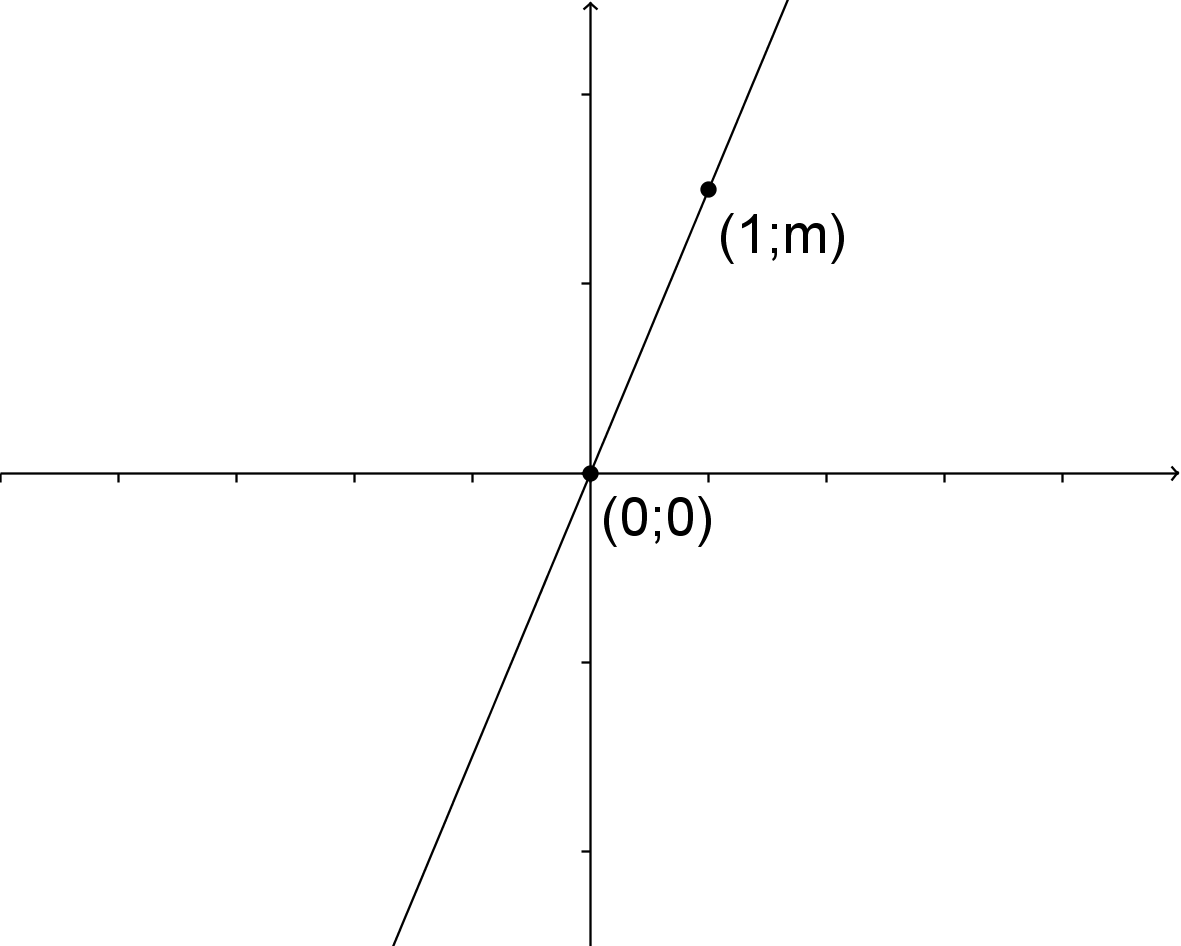
\includegraphics[height=4cm]{../images/005_direct_propp}
	\caption{Egyenes arányosság} 
\end{figure}
\end{defin}

\begin{defin}[Fordított arányosság]
$x$ és $y$ változó valós mennyiségek között \dashuline{fordított arányosság}
áll fenn, ha a két változó mennyiség összetartozó, nullától különböző
értékeinek szorzata nullától különböző állandó, azaz:
\[
xy = c
\]
ahol $x \neq 0$, $y \neq 0$, $c \neq 0$. $c$ az ún. arányossági tényező.

A fordított arányossághoz tartozó függvény grafikonja hiperbola.

\begin{figure}[!h]
	\centering
	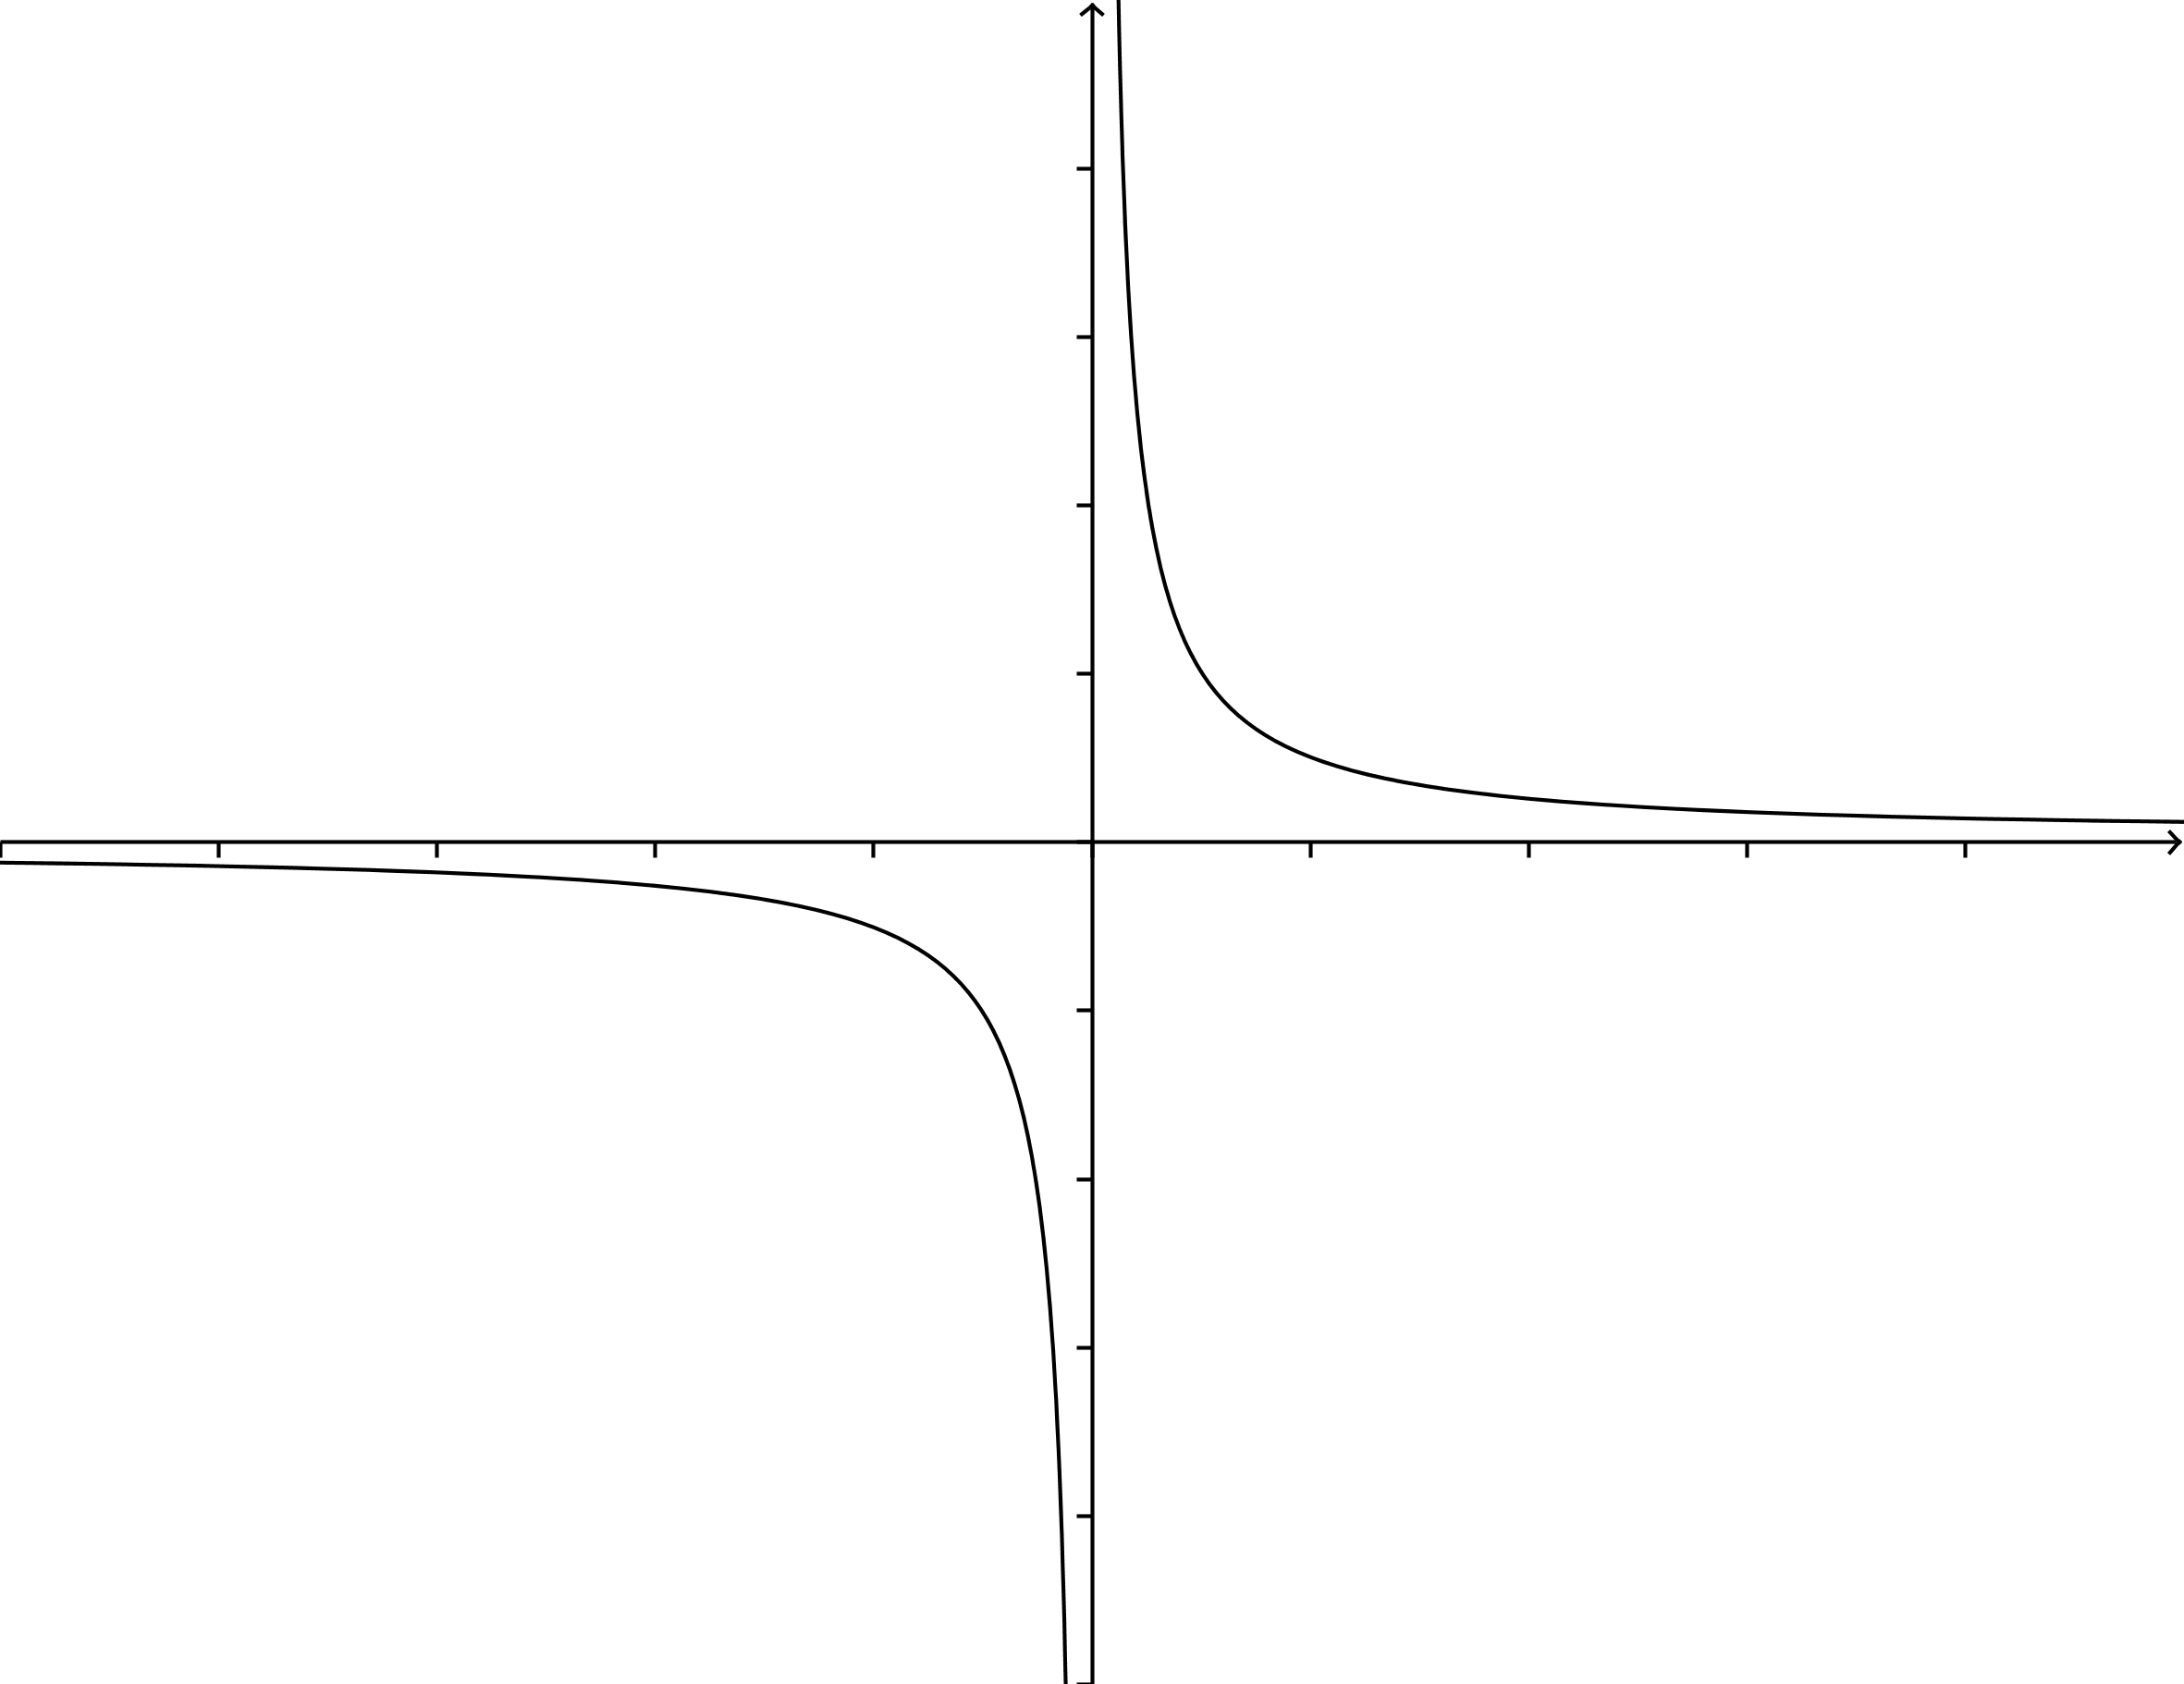
\includegraphics[height=4cm]{../images/005_indirect_propp}
	\caption{Fordított arányosság} 
	\label{fig:inverserate}
\end{figure}
\end{defin}

\textbf{Lásd még:}
